% В этом файле следует писать текст работы, разбивая его на
% разделы (section), подразделы (subsection) и, если нужно,
% главы (chapter).

% Предварительно следует указать необходимую информацию
% в файле SETUP.tex

%% В этот файл не предполагается вносить изменения

% В этом файле следует указать информацию о себе
% и выполняемой работе.

\documentclass [fontsize=14pt, paper=a4, pagesize, DIV=calc]%
{scrartcl}
% ВНИМАНИЕ! Для использования глав поменять
% scrartcl на scrreprt

% Здесь ничего не менять
\usepackage [T2A] {fontenc}   % Кириллица в PDF файле
\usepackage [utf8] {inputenc} % Кодировка текста: utf-8
\usepackage [russian] {babel} % Переносы, лигатуры

%%%%%%%%%%%%%%%%%%%%%%%%%%%%%%%%%%%%%%%%%%%%%%%%%%%%%%%%%%%%%%%%%%%%%%%%
% Создание макроса управления элементами, специфичными
% для вида работы (курс., бак., маг.)
% Здесь ничего не менять:
\usepackage{ifthen}
\newcounter{worktype}
\newcommand{\typeOfWork}[1]
{
	\setcounter{worktype}{#1}
}

% ВНИМАНИЕ!
% Укажите тип работы: 0 - курсовая, 1 - бак., 2 - маг.,
% 3 - бакалаврская с главами.
\typeOfWork{1}
% Считается, что курсовая и бак. бьются на разделы (section) и
% подразделы (subsection), а маг. — на главы (chapter), разделы и
%  подразделы. Если хочется,
% чтобы бак. была с главами (например, если она большая),
% надо выбрать опцию 3.

% Если при выборе 2 или 3 вы забудете поменять класс
% документа на scrreprt (см. выше, в самом начале),
% то получите ошибку:
% ./aux/appearance.tex:52: Package scrbase Error: unknown option ` chapterprefix=

%%%%%%%%%%%%%%%%%%%%%%%%%%%%%%%%%%%%%%%%%%%%%%%%%%%%%%%%%%%%%%%%%%%%%%%%
% Информация об авторе и работе для титульной страницы

\usepackage {titling}

% Имя автора в именительном падеже (для маг.)
\newcommand {\me}{%
Е.\,А.~Тактаров%
}

% Имя автора в родительном падеже (для курсовой и бак.)
\newcommand {\byme}{%
Е.\,А.~Тактарова%
}

% Научный руководитель
\newcommand{\supervisor}%
{к.ф.-м.н., доцент Е. М. Андреева}

% идентифицируем пол (только для курсовой и бак.)
\newcommand{\bystudent}{
Студента %Студентки % Для курсовой: с большой буквы
}

% Год публикации
\date{2019}

% Название работы
\title{Разработка системы проведения опросов аудитории\\ во время публичных выступлений}

% Кафедра
%

\newcommand {\direction} {%
Направление подготовки\\02.\ifthenelse{\value{worktype} = 2}{04}{03}.02 ---
Фундаментальная информатика\\и информационные технологии%
}

%%%%%%%%%%%%%%%%%%%%%%%%%%%%%%%%%%%%%%%%%%%%%%%%%%%%%%%%%%%%%%%%%%%%%%%%
% Другие настраиваемые элементы текста

% Листинги с исходным кодом программ: укажите язык программирования
\usepackage{listings}
\lstset{
    language=[ISO]C++,%  Язык указать здесь
    basicstyle=\small\ttfamily,
    breaklines=true,%
    showstringspaces=false%
    inputencoding=utf8x%
}
% полный список языков, поддерживаемых данным пакетом, есть,
% например, здесь (стр. 13):
% ftp://ftp.tex.ac.uk/tex-archive/macros/latex/contrib/listings/listings.pdf

\usepackage{color}
\definecolor{lightgray}{rgb}{.9,.9,.9}
\definecolor{darkgray}{rgb}{.4,.4,.4}
\definecolor{purple}{rgb}{0.65, 0.12, 0.82}
\lstdefinelanguage{JavaScript}{
	keywords={break, case, catch, continue, debugger, default, delete, do, else, false, finally, for, function, if, in, instanceof, new, null, return, switch, this, throw, true, try, typeof, var, void, while, with},
	morecomment=[l]{//},
	morecomment=[s]{/*}{*/},
	morestring=[b]',
	morestring=[b]",
	ndkeywords={class, export, boolean, throw, implements, import, this,require},
	keywordstyle=\color{blue}\bfseries,
	ndkeywordstyle=\color{cyan}\bfseries,
	identifierstyle=\color{black},
	commentstyle=\color{purple}\ttfamily,
	stringstyle=\color{red}\ttfamily,
	sensitive=true
}


\usepackage{xcolor}

\colorlet{punct}{red!60!black}
\definecolor{background}{HTML}{EEEEEE}
\definecolor{delim}{RGB}{20,105,176}
\colorlet{numb}{magenta!60!black}

\lstdefinelanguage{json}{
	basicstyle=\normalfont\ttfamily,
	numbers=left,
	numberstyle=\scriptsize,
	stepnumber=1,
	numbersep=8pt,
	showstringspaces=false,
	breaklines=true,
	frame=lines,
	backgroundcolor=\color{background},
	literate=
	*{0}{{{\color{numb}0}}}{1}
	{1}{{{\color{numb}1}}}{1}
	{2}{{{\color{numb}2}}}{1}
	{3}{{{\color{numb}3}}}{1}
	{4}{{{\color{numb}4}}}{1}
	{5}{{{\color{numb}5}}}{1}
	{6}{{{\color{numb}6}}}{1}
	{7}{{{\color{numb}7}}}{1}
	{8}{{{\color{numb}8}}}{1}
	{9}{{{\color{numb}9}}}{1}
	{:}{{{\color{punct}{:}}}}{1}
	{,}{{{\color{punct}{,}}}}{1}
	{\{}{{{\color{delim}{\{}}}}{1}
	{\}}{{{\color{delim}{\}}}}}{1}
	{[}{{{\color{delim}{[}}}}{1}
	{]}{{{\color{delim}{]}}}}{1},
}




% Нумерация списков: можно при необходимести
% изменять вид нумерации (например, добавлять правую скобку).
% По умолчанию буду списки вида:
% 1.
% 2.
% Изменять вид нумерации можно в начале нумерации:
% \begin{enumerate}[1)] (В квадратных скобках указан желаемый вид)
\usepackage[shortlabels]{enumitem}
                    \setlist[enumerate, 1]{1.}

% Гиперссылки: настройте внешний вид ссылок
\usepackage%
[pdftex,unicode,pdfborder={0 0 0},draft=false,%backref=page,
    hidelinks, % убрать, если хочется видеть ссылки: это
               % удобно в PDF файле, но не должно появиться на печати
    bookmarks=true,bookmarksnumbered=false,bookmarksopen=false]%
{hyperref}


\usepackage {amsmath}      % Больше математики
\usepackage {amssymb}
\usepackage {textcase}     % Преобразование к верхнему регистру
\usepackage {indentfirst}  % Красная строка первого абзаца в разделе

\usepackage {fancyvrb}     % Листинги: определяем своё окружение Verb
\DefineVerbatimEnvironment% с уменьшенным шрифтом
	{Verb}{Verbatim}
	{fontsize=\small}

% Вставка рисунков
\usepackage {graphicx}

% Общее оформление
% ----------------------------------------------------------------
% Настройка внешнего вида

%%% Шрифты

% если закомментировать всё — консервативная гарнитура Computer Modern
\usepackage{paratype} % профессиональные свободные шрифты
%\usepackage {droid}  % неплохие свободные шрифты от Google
%\usepackage{mathptmx}
%\usepackage {mmasym}
%\usepackage {psfonts}
%\usepackage{lmodern}
%var1: lh additions for bold concrete fonts
%\usepackage{lh-t2axccr}
%var2: the package below could be covered with fd-files
%\usepackage{lh-t2accr}
%\usepackage {pscyr}

% Геометрия текста

\usepackage{setspace}       % Межстрочный интервал
\onehalfspacing

\newlength\MyIndent
\setlength\MyIndent{1.25cm}
\setlength{\parindent}{\MyIndent} % Абзацный отступ
\frenchspacing            % Отключение лишних отступов после точек
\KOMAoptions{%
    DIV=calc,         % Пересчёт геометрии
    numbers=endperiod % точки после номеров разделов
}

                            % Консервативный вариант:
%\usepackage                % ручное задание геометрии
%[%                         % (не рекомендуется в проф. типографии)
%  margin = 2.5cm,
  %includefoot,
  %footskip = 1cm
%] %
%  {geometry}

%%% Заголовки


\ifthenelse{{\value{worktype} > 1}}{%
  \KOMAoptions{%
      headings=normal,   % размеры заголовков поменьше стандартных
      chapterprefix=true,% Печатать слово Глава
      appendixprefix=true% Печатать слово Приложение
  }
}{% Печатать слово Приложение даже если нет глав
  \newcommand*{\appendixmore}{%
    \renewcommand*{\sectionformat}{%
    \appendixname~\thesection\autodot\enskip}
    \renewcommand*{\sectionmarkformat}{%
      \appendixname~\thesection\autodot\enskip}
  }
}

% шрифт для оформления глав и названия содержания
\newcommand{\SuperFont}{\Large\sffamily\bfseries}

% Заголовок главы
\ifthenelse{\value{worktype} > 1}{%
\renewcommand{\SuperFont}{\Large\normalfont\sffamily}
\newcommand{\CentSuperFont}{\centering\SuperFont}
\usepackage{fncychap}
\ChNameVar{\SuperFont}
\ChNumVar{\CentSuperFont}
\ChTitleVar{\CentSuperFont}
\ChNameUpperCase
\ChTitleUpperCase
}

% Заголовок (под)раздела с абзацного отступа
\addtokomafont{sectioning}{\hspace{\MyIndent}}

\renewcommand*{\captionformat}{~---~}
\renewcommand*{\figureformat}{Рисунок~\thefigure}

% Плавающие листинги
\usepackage{float}
\floatstyle{ruled}
\floatname{ListingEnv}{Листинг}
\newfloat{ListingEnv}{htbp}{lol}[section]

% точка после номера листинга
\makeatletter
\renewcommand\floatc@ruled[2]{{\@fs@cfont #1.} #2\par}
\makeatother


%%% Оглавление
\usepackage{tocloft}

% шрифт и положение заголовка
\ifthenelse{\value{worktype} > 1}{%
\renewcommand{\cfttoctitlefont}{\hfil\SuperFont\MakeUppercase}
}{
\renewcommand{\cfttoctitlefont}{\hfil\SuperFont}
}

% слово Глава
\usepackage{calc}
\ifthenelse{\value{worktype} > 1}{%
\renewcommand{\cftchappresnum}{Глава }
\addtolength{\cftchapnumwidth}{\widthof{Глава }}
}

% Очищаем оформление названий старших элементов в оглавлении
\ifthenelse{\value{worktype} > 1}{%
\renewcommand{\cftchapfont}{}
\renewcommand{\cftchappagefont}{}
}{
\renewcommand{\cftsecfont}{}
\renewcommand{\cftsecpagefont}{}
}

% Точки после верхних элементов оглавления
\renewcommand{\cftsecdotsep}{\cftdotsep}
%\newcommand{\cftchapdotsep}{\cftdotsep}

\ifthenelse{\value{worktype} > 1}{%
    \renewcommand{\cftchapaftersnum}{.}
}{}
\renewcommand{\cftsecaftersnum}{.}
\renewcommand{\cftsubsecaftersnum}{.}
\renewcommand{\cftsubsubsecaftersnum}{.}

%%% Списки (enumitem)

\usepackage {enumitem}      % Списки с настройкой отступов
\setlist %
{ %
  leftmargin = \parindent, itemsep=.5ex, topsep=.4ex
} %

% По ГОСТу нумерация должны быть буквами: а, б...
%\makeatletter
%    \AddEnumerateCounter{\asbuk}{\@asbuk}{м)}
%\makeatother
%\renewcommand{\labelenumi}{\asbuk{enumi})}
%\renewcommand{\labelenumii}{\arabic{enumii})}

%%% Таблицы: выбрать более подходящие

\usepackage{booktabs} % считаются наиболее профессионально выполненными
%\usepackage{ltablex}
%\newcolumntype {L} {>{---}l}

%%% Библиография

\usepackage{csquotes}        % Оформление списка литературы
\usepackage[
  backend=biber,
  hyperref=auto,
  sorting=none, % сортировка в порядке встречаемости ссылок
  language=auto,
  citestyle=gost-numeric,
  bibstyle=gost-numeric
]{biblatex}
\addbibresource{biblio.bib} % Файл с лит.источниками

% Настройка величины отступа в списке
\ifthenelse{\value{worktype} < 2}{%
\defbibenvironment{bibliography}
  {\list
     {\printtext[labelnumberwidth]{%
    \printfield{prefixnumber}%
    \printfield{labelnumber}}}
     {\setlength{\labelwidth}{\labelnumberwidth}%
      \setlength{\leftmargin}{\labelwidth}%
      \setlength{\labelsep}{\dimexpr\MyIndent-\labelwidth\relax}% <----- default is \biblabelsep
      \addtolength{\leftmargin}{\labelsep}%
      \setlength{\itemsep}{\bibitemsep}%
      \setlength{\parsep}{\bibparsep}}%
      \renewcommand*{\makelabel}[1]{\hss##1}}
  {\endlist}
  {\item}
}{}

% ----------------------------------------------------------------
% Настройка переносов и разрывов страниц

\binoppenalty = 10000      % Запрет переносов строк в формулах
\relpenalty = 10000        %

\sloppy                    % Не выходить за границы бокса
%\tolerance = 400          % или более точно
\clubpenalty = 10000       % Запрет разрывов страниц после первой
\widowpenalty = 10000      % и перед предпоследней строкой абзаца

% ----------------------------


% Стили для окружений типа Определение, Теорема...
% Оформление теорем (ntheorem)

\usepackage [thmmarks, amsmath] {ntheorem}
\theorempreskipamount 0.6cm

\theoremstyle {plain} %
\theoremheaderfont {\normalfont \bfseries} %
\theorembodyfont {\slshape} %
\theoremsymbol {\ensuremath {_\Box}} %
\theoremseparator {:} %
\newtheorem {mystatement} {Утверждение} [section] %
\newtheorem {mylemma} {Лемма} [section] %
\newtheorem {mycorollary} {Следствие} [section] %

\theoremstyle {nonumberplain} %
\theoremseparator {.} %
\theoremsymbol {\ensuremath {_\diamondsuit}} %
\newtheorem {mydefinition} {Определение} %

\theoremstyle {plain} %
\theoremheaderfont {\normalfont \bfseries} 
\theorembodyfont {\normalfont} 
%\theoremsymbol {\ensuremath {_\Box}} %
\theoremseparator {.} %
\newtheorem {mytask} {Задача} [section]%
\renewcommand{\themytask}{\arabic{mytask}}

\theoremheaderfont {\scshape} %
\theorembodyfont {\upshape} %
\theoremstyle {nonumberplain} %
\theoremseparator {} %
\theoremsymbol {\rule {1ex} {1ex}} %
\newtheorem {myproof} {Доказательство} %

\theorembodyfont {\upshape} %
%\theoremindent 0.5cm
\theoremstyle {nonumberbreak} \theoremseparator {\\} %
\theoremsymbol {\ensuremath {\ast}} %
\newtheorem {myexample} {Пример} %
\newtheorem {myexamples} {Примеры} %

\theoremheaderfont {\itshape} %
\theorembodyfont {\upshape} %
\theoremstyle {nonumberplain} %
\theoremseparator {:} %
\theoremsymbol {\ensuremath {_\triangle}} %
\newtheorem {myremark} {Замечание} %
\theoremstyle {nonumberbreak} %
\newtheorem {myremarks} {Замечания} %


% Титульный лист
% Макросы настройки титульной страницы
% В этот файл не предполагается вносить изменения

%\usepackage {showframe}

% Вертикальные отступы на титульной странице
\newcommand{\vgap}{\vspace{16pt}}

% Помещение города и даты в нижний колонтитул
\usepackage{scrlayer}
\DeclareNewLayer[
  foot,
  foreground,
  contents={%
    \raisebox{\dp\strutbox}[\layerheight][0pt]{%
      \parbox[b]{\layerwidth}{\centering Ростов-на-Дону\\ \thedate%
       \\\mbox{}
       }}%
  }
]{titlepage.foot.fg}
\DeclareNewPageStyleByLayers{titlepage}{titlepage.foot.fg}


\AtBeginDocument %
{ %
  %
  \begin{titlepage}
  %
    \thispagestyle{titlepage}

    {\centering
    %
    \MakeTextUppercase {МИНИСТЕРСТВО ОБРАЗОВАНИЯ И НАУКИ РФ}

    \vgap

    Федеральное государственное автономное образовательное\\
    учреждение высшего образования\\
    \MakeTextUppercase {Южный федеральный университет}

    \vgap

	Институт математики, механики и компьютерных наук
    имени~И.\,И.\,Воровича

    \vgap

    \direction

    \vspace* {\fill}

    \ifthenelse{\value{worktype} = 2}{%
    \me

    \vgap}{}

    {\usefont{T2A}{PTSansCaption-TLF}{m}{n}
    \MakeTextUppercase{\thetitle}}

    \ifthenelse{\value{worktype} = 2}{%
     \vgap

    Магистерская диссертация}{}
    \ifthenelse{\value{worktype} = 0}{
     \vgap

    Курсовая работа
    }{}%
    \ifthenelse{\value{worktype} = 1 \OR \value{worktype} = 3}{
     \vgap

    Выпускная квалификационная работа\\
    на степень бакалавра
    }{}%

    \vspace {\fill}

    \begin{flushright}
    \ifthenelse{\value{worktype} = 0 \OR 
                \value{worktype} = 1 \OR
                \value{worktype} = 3}{
      \bystudent \ifthenelse{\value{worktype} = 0}{3}{4}\ курса\\
      \byme
    }{}

    \vgap

    Научный руководитель:\\
    \supervisor\\
    \ifthenelse{\value{worktype} = 2}{%
    Рецензент:\\
    ученая степень, ученое звание, должность
    И. О. Фамилия
    }{}
	\end{flushright}
\ifthenelse{\value{worktype} = 0}{
\vspace{\fill}
        \begin{flushleft}
          \begin{tabular}{cc}
            \underline{\hspace{4cm}}&\underline{\hspace{5cm}}\\
            {\small оценка (рейтинг)} & {\small  подпись руководителя}\\
          \end{tabular}
          \\[1cm]
        \end{flushleft}
}{}
\ifthenelse{\value{worktype} = 1 \OR \value{worktype} = 3}{
\vspace{\fill}
        \begin{flushleft}
Допущено к защите:\\руководитель направления ФИИТ
\underline{\hspace{4cm}}
В.\,С.\,Пилиди
        \end{flushleft}
}{}


  	\vspace {\fill}
  %Ростов-на-Дону

    %\thedate

  }\end{titlepage}
  %
  %
  \tableofcontents
  %
  \clearpage
} %


% Команды для использования в тексте работы


% макросы для начала введения и заключения
\newcommand{\Intro}{\addsec{Введение}}
\ifthenelse{\value{worktype} > 1}{%
    \renewcommand{\Intro}{\addchap{Введение}}%
}

\newcommand{\Conc}{\addsec{Заключение}}
\ifthenelse{\value{worktype} > 1}{%
    \renewcommand{\Conc}{\addchap{Заключение}}%
}

% Правильные значки для нестрогих неравенств и пустого множества
\renewcommand {\le} {\leqslant}
\renewcommand {\ge} {\geqslant}
\renewcommand {\emptyset} {\varnothing}

% N ажурное: натуральные числа
\newcommand {\N} {\ensuremath{\mathbb N}}

% значок С++ — используйте команду \cpp
\newcommand{\cpp}{%
C\nolinebreak\hspace{-.05em}%
\raisebox{.2ex}{+}\nolinebreak\hspace{-.10em}%
\raisebox{.2ex}{+}%
}

% Неразрывный дефис, который допускает перенос внутри слов,
% типа жёлто-синий: нужно писать жёлто"/синий.
\makeatletter
    \defineshorthand[russian]{"/}{\mbox{-}\bbl@allowhyphens}
\makeatother


\endinput

% Конец файла



\NewBibliographyString{langjapanese}
\NewBibliographyString{fromjapanese}

\begin{document}

\Intro
Технологии проведения публичных выступлений и презентаций затрагивают навыки ораторства и внешний вид, дизайн медиа-сопровождения. Методы взаимодействия с аудиторией традиционно включают в первую составляющую. Выступающий, желающий взаимодействовать со слушающими, должен уже обладать определенным опытом в работе с ними и ограничен устными средствами.Крайне редко возможно почти полностью вовлечь аудиторию в выступление, ведь лишь немногие слушатели готовы,например, задать вопрос или ответить выступающему.


Распространение телефонов и мобильного доступа в интернет, позволяет использовать эти устройства как средства взаимодействия с аудиторией. Проекты, использующие эту идею, реализовывались неоднократно, но ни один из них не закрепился как широко используемый в публичных выступлениях. В первую очередь, идея взаимодействия с публикой через телефоны реализовывалась под конкретные единичные выступления. Последующие реализации, хотя и обладают обширным функционалом, в виде  опросов, голосований и чатов, представлют собой отдельные веб-сервисы, направленные на монетизацию с пользователей. Все проекты закрыты проприетарными лицензиями и требуют от пользователей загрузки презентации на сторонний сервер.

Данная работа посвящена разработке проекта портативного веб-сервиса под свободной лицензией, который позволит проводить опросы аудитории во время публичных выступлений без привлечения сторонних сервисов. Свободная лицензия позволит любому человеку изменять и расширять возможности сервиса под свои нужды.

Задача по созданию такого проекта включает разработку как веб-интерфейса пользователя (фронтенд), так и  внутренней логики сервиса(бэкенд), которые в совокупности обеспечат динамичное отображение результатов опросов.
   
\section{Исследование предметной области}
\subsection{Обзор существующих решений}
Как и упоминалось ранее, для опросов аудитории уже существует немалое число инструментов, однако в основой массе это закрытые решения в виде веб-сервисов:
\begin{itemize}
	\item polleverywhere.com
	\item directpoll.com
	\item sli.do
	\item ficus.io
\end{itemize}
На этих сайтах и других подобных можно бесплатно в первый раз провести опрос или даже презентацию, но повторные показы и дополнительные функции ограничены для пользователей, не оплативших услуги сайтов. Более того, даже оплативший пользователь ограничен средствами и функциями сайта и не может модифицировать или изменить инструмент под свои нужды и цели.

Также стоит упомянуть об инструментах опросов, не использующих только Интернет(http://www.ombea.com/). Такие решения применяются в университетах США(http://www.nea.org/home/34690.html) и отличаются низкой способностью к масштабированию и высокой ценной как системы, так и индивидуальных приборов голосования.

\subsection{Обзор инструментов разработки}
При создании веб-сервиса самую важную роль занимает разработка серверной части. Так как веб-сайт должен динамически взаимодействовать с сервером, то архаичная связка из веб-сервера и FastCGI/CGI приложения очевидно не подойдет. Для решения данной задачи необходимо выбрать один из множества современных веб-фреймворков (https://ru.wikipedia.org/wiki/Сравнение\_каркасов\_веб-приложений), как основу для проекта. Отметим основные необходимые для задачи черты фреймворков:
 \begin{itemize}
 	\item легковесность
 	\item инкапсуляция веб-сервера
 	\item наличие актуального функционала(JSON,AJAX,websocket)
 \end{itemize}
Рассмотрим несколько популярных фреймворков:
 \begin{itemize}
 	\item Django --- фреймворк на языке Python. Хотя на нем можно реализовать необходимый нам функционал, но его врядли можно назвать легковесным. Django в первую очередь предназначен для создания больших многостраничных сайтов и сервисов, которые будет длительное время поддерживать команда разработчиков и администраторов. Наличие бесполезного для задачи функционалла негативно сказывается на времени освоения и разработки. (https://www.djangoproject.com/)  
 	\item Ruby on Rails --- фреймворк на языке Ruby. Основными минусами Ruby on Rails являются проксирование через отдельный веб-сервер и общая сложность освоения как фреймворка, так и самого языка.Стоит также отметить, что этот фреймворк сильно опирается на архитектуру модель-представление-контроллер, реализация которой усложняет задачу для небольшого приложения.  (https://rubyonrails.org/)  
 	\item Express --- фреймворк на языке Javasciprt, запускаемый на платоформе Node.js. Express  инкапсулирует веб-сервер,представляя только абстракцию в виде объектов HTTP запроса и ответа,а необходимый для приложения функционал, например WebSocket и шаблонизация , добавляются через совместимы модули Node.js. Так же фреймворк не затрагивает клиентскую часть веб-приложения.(https://expressjs.com/ru/) Express своевременно обновляется, имеет обширную документацию и является популярным выбором среди разработчиков из-за своей простоты и понятности. Основным опасением является производительность однопоточной архитектуры Node.js, однако для небольших и средних приложений Node.js и Express показывают удовлетворительные результаты(https://www.researchgate.net/publication/286594024\_Performance\_Comparison\_and\_Evaluation\_of\_Web\_Development\_Technologies\_in\_PHP\_Python\_and\_Nodejs) 
 \end{itemize}
Таким образом, для решения рассматриваемой задачи фреймворк Express подходит идеально. Так как он не затрагивает клиентскую часть сервиса, то для нее можно использовать любой легковесный JavaScript фреймворк для создания пользовательского интерфейса.

Также важно выбрать технологию обмена данных между сервером и клиентом. Так как в нашем случае сервер должен отправлять данные, даже когда клиент не запрашивает их явно, то данное веб-приложение соотвествует модели COMET ( Krill, Paul (September 24, 2007). "AJAX alliance recognizes mashups". InfoWorld. Retrieved 2010-10-20.). Рассмотрим некоторые технологии реализации COMET в современных веб-приложениях:

\begin{description}
	\item[Спрятанный iframe] Iframe HTML-элемент, который подгружает "бесконечную" под-страницу с сервера, состоящую из элементов script с данными. Такой метод, требует особой модификации веб-сервера, но поддерживается во всех браузерах. Достаточно сложен в реализации как на сервере, так и на клиенте. 
	\item[подгружаемый XMLHttpRequest] аналогично с предыдущим методом, но вместо страницы загружается AJAX-запрос.
	\item[XMLHttpRequest long polling] в этой технологии браузер отправляет AJAX-запрос, но ответ получает, только когда серверу нужно отправить данные клиенту. 
	\item[WebSocket] отдельный протокол двустороннего соединения поверх TCP. Его реализация есть во всех современных браузерах и серверах, в том числе и для Node.js. По сравнению с другими технологиями WebSocket отличается производительностью, скоростью передачи данных и удобством в работе.
\end{description}
Исходя из этого, для данной задачи лучше всего использовать технологию WebSocket.

 
\section{Обзор Проекта}
Решение поставленной задачи будет представлено в виде веб-сервиса на фреймворке Express на Node.js, имеющего следующие отличительные функции и особенности:
 \begin{itemize}
	\item Создание и проведение опросов. 
	\item Динамическое отображение результатов опроса на странице.
	\item Каждый опрос имеет короткие ссылки для голосования и просмотра результатов.
	\item Параллельное проведение нескольких опросов на одном веб-сервисе.
	\item Защита от вредоносного искажения результатов. 
	\item Взаимодействие клиента и сервера через технологию WebSocket.
	\item Открытый исходный код под свободной лицензией.
\end{itemize} 
 
\section{Аспекты реализации}
\subsection{Структура проекта на Node.js}
\label{subsec:project_structuture}
Для создания основы проекта на с использованием Express я использовал генератор проектов express-generator (https://www.npmjs.com/package/express-generator) . Эта утилита позволяет избавится от необходимости конфигурировать встроенный сервер и параметры фреймворка. После ее выполнения в выбранном каталоге генерируется простое, готовое для запуска  веб-приложение вот такой структуры:
\dirtree{%
.1 sample-app.
.2 app.js.
.2 bin.
.3 www.
.2 package.json.
.2 public.
.3 images.
.3 javascripts.
.3 stylesheets.
.4 style.css.
.2 routes.
.3 index.js.
.3 users.js.
.2 views.
.3 error.pug.
.3 index.pug.
.3 layout.pug.
}    
 Разберем назначение некоторых файлов и каталогов:
 \begin{description}
 	\item[package.json] файл с указаниями для пакетного менеджера npm для Node.js. Содержит список всех пакетов, от которых зависит приложение, и точку входа для Node.js.  
 	\item[bin/www] точка входа исполняемого кода Javascript. В нем создаются и соединяются объекты HTTP-сервера и Express-приложения. Все остальные файлы кода для Node.js являются Javascipts-модулями, которые подключаются в www, либо в других модулях, уже подключенных в www.
 	\item[app.js] файл с настройками, касающихся конкретно работы Express.Также в нем подключаются файлы с обработчиками путей запросов.   
 	\item[public/] в настройках проекта этот каталог, сконфигурирован как общедоступный для  HTTP-запросов вида GET. В нем хранятся статичные файлы для клиентской части веб-сервиса. Во время его работы эти файлы доступны по запросам вида http://project.com/stylesheets/style.css.
 	\item[routes/]   содержит обработчики путей запросов, поступающих в Express.
 	\item[views/]   содержит файлы шаблоны веб-страниц в формате PUG.  
 \end{description}


Такой шаблон проекта значительно упростил разработку сервиса, потому что любой написанный поверх него функционал сразу можно запустить и протестировать, а готовое файловое устройство принуждает к структурированному стилю написания кода. В конечном проекте структура каталогов приложения остается такой же, а только изменяются и добавляются в них файлы кода.      
\subsection{Использование фреймворка Express}
Разработка веб-сервиса на Express сводится к написанию обработчиков путей HTTP-запросов поступающих на сервер.
\begin{ListingEnv}[H]
\begin{lstlisting}
router.get("/get_polled",function(req, res, next){
 let id = db.create_polling_session({
	title: "poll",
	options: [
	  { title: "option1" },
	  { title: "option2" },
	  { title: "option3" }
 ]});
 res.status(200).json({link:db.polling_sessions[id].view_link});
});
	
\end{lstlisting}
\caption{Пример функции обработчика GET-запроса}
\label{list:routing_example}
\end{ListingEnv}
В примере (листинг~\ref{list:routing_example}) для объекта router, который затем можно экспортировать для использовании в приложении Express, определяется поведение при поступлении GET-запроса по адресу sample.com/get\_polled. Для этого используется анонимная функция обратного вызова, которая исполняется каждый раз при поступлении запроса. Аргументы req, res, next представляют, соотвественно, объекты с данными о запросе(REQuest), с функциями ответа (RESponse) и функцию для вызова следующего подходящего обработчика пути. В примере происходит взаимодействие с моделью данных и отправка клиенту ответа с результатами взаимодействия в формате JSON.

Стоит отметить, что возможность использовать регулярные выражения и сопоставление с образцом в для путей запросов, а также выстраивать цепочки из обработчиков позволило выстроить в веб-сервисе относительно сложную логику ответов на запросы. Хотя описание этой логики в исходном коде не занимает много места.  

\subsection{Использование WebSocket совместно с фреймворком Express}
Для того чтобы добавить функциональность WebSocket в приложение, я воспользовался пакетом express-ws (https://www.npmjs.com/package/express-ws). Этот пакет добавляет в Express функцию для создания обработчиков путей запроса соединения по протоколу WebSocket. Чтобы добавить желаемый функционал код из пакета модифицирует прототипы класса Router внутри Express и добавляет в указанный веб-сервер обработчик запросов типа:
\begin{lstlisting}[language]
GET /exmpl HTTP/1.1
Host: server.example.com
Upgrade: websocket
Connection: Upgrade
...
\end{lstlisting}
После этого в контексте фреймворка можно писать обработчики путей для WebSocket:
\begin{ListingEnv}[H]
	\begin{lstlisting}
app.ws('/echo', function(ws, req) {
	ws.on('message', function(msg) {
		ws.send(msg);
	});
});
	\end{lstlisting}
	\caption{Пример функции обработчика WS-запроса}
	\label{list:ws_example}
\end{ListingEnv}
В примере (листинг~\ref{list:ws_example}) в отличии от примера в листинге~\ref{list:routing_example} нет объекта ответа res,но есть объект ws --- асинхронно открывающийся вебсокет, представляющий соединение между конкретным клиентом и сервером. К этому объекту уже можно привязать функции обработчики для событий изменения состояния вебсокета или получения данных. Когда состояние вебсокета изменится на OPEN, для объекта ws можно вызвать метод send и отправить клиенту любые данные.   

Как было сказано в подразделе~\ref{subsec:project_structuture} в шаблоне express-generator создание объекта HTTP-сервера и связывание его с экземпляром объекта Express происходит в файле bin/www, который является входной точкой исполнения кода для Node.js. Такое устройство приложения по-умолчанию не подходит для express-ws, которому нужно вмешаться в устройство сервера и экземпляра Express. Чтобы это исправить, необходимо внести определенные изменения в файлы app.js и bin/www.

Пользуясь тем, что app.js импортируется в начале www/bin, а значит и интерпретируется раньше чем его основной код, я перенес создание экземпляров HTTP-сервера и Express в app.js. Там же происходит внедрение express-ws.
\begin{ListingEnv}[H]
\begin{lstlisting}
	...
var express = require('express');
var http = require('http');
	...
var app = express();
app.server = http.createServer(app); 
var expressWS = require('express-ws')(app, app.server);
	...
module.exports = app;
\end{lstlisting}
\caption{Изменения в app.js}
\label{list:appjs-ws}
\end{ListingEnv}  
Внутри bin/www создание сервера я заменил на обращение к ссылке на веб-сервер из экземпляра Express.
\begin{ListingEnv}[H]
\begin{lstlisting}
var app = require('../app');
	...
var server = app.server;
server.listen(port);
server.on('error', onError);
server.on('listening', onListening);
	...
\end{lstlisting}
\caption{Изменения в bin/www}
\label{list:www-ws}
\end{ListingEnv}

Таким образом, возможно воспользоваться технологией WebSocket, не нарушая структуру шаблонного приложения на фреймворке Express. 

\subsection{Проектирование модели данных}

 
 
 
 
 
 
 
   
% Если typeOfWork в SETUP.tex задан как 2 или 3, то начинать
% надо не с section (раздел), а с главы (chapter)
\section{Несколько примеров в~\LaTeX{}}
\label{sec:examples}

Некоторые часто используемые
команды приведены в качестве примера ниже (и варианты — в
комментариях). Мы рекомендуем внимательно прочесть данный
текст и изучить его исходный код прежде, чем начинать писать
свой собственный. Кроме того, можно дать и такой совет: идущий
ниже текст не убирать до самого конца, а просто оставлять его
позади своего собственного текста, чтобы в любой момент можно
было проконсультироваться с данными примерами.

\subsection{Как вставлять листинги и рисунки}

Для крупных листингов есть два способа. Первый красивый, но в нём не допускается
кириллица (у вас может встречаться в комментариях и
печатаемых сообщениях), он представлен на листинге~\ref{list:hwbeauty}.
\begin{ListingEnv}[H]% буква H означает Here, ставим здесь,
% элементы, которые нежелательно разрывать обычно не ставят
% посреди страницы: вместо H используется t (top, сверху страницы),
% или b (bottom) или p (page, на отдельной странице)
\begin{lstlisting}
#include <iostream>
using namespace std;

int main()
{
    cout << "Hello, world" << endl;
    system("pause");
    return 0;
}
\end{lstlisting}
%следующую команду для генерации подписи можно опустить,
% хотя рекомендуется все специальные элементы (таблицы, рисунки,
% листинги) подписывать. Если подпись пропустить, листинг также не получит
% номера и на него не сошлёшься в будущем
\caption{Программа “Hello, world” на \protect\cpp}
% далее метка для ссылки:
\label{list:hwbeauty}
\end{ListingEnv}

Второй не такой красивый, но без ограничений (см.~листинг~\ref{list:hwplain}).
\begin{ListingEnv}[H]
\begin{Verb}

#include <iostream>
using namespace std;

int main()
{
    cout << "Привет, мир" << endl;
}
\end{Verb}
\caption{Программа “Hello, world” без подсветки}
\label{list:hwplain}
\end{ListingEnv}

Можно использовать первый для вставки небольших фрагментов
внутри текста, а второй для вставки полного
кода в приложении, если таковое имеется.

Если нужно вставить совсем короткий пример кода (одна или две строки), то выделение  линейками и нумерация может смотреться чересчур громоздко. В таких случаях можно использовать окружения \texttt{lstlisting} или \texttt{Verb} без \texttt{ListingEnv}. Приведём такой пример с указанием языка программирования, отличного от заданного по умолчанию:
\begin{lstlisting}[language=Haskell]
fibs = 0 : 1 : zipWith (+) fibs (tail fibs)
\end{lstlisting}
Такое решение~--- со вставкой нумерованных листингов покрупнее
и вставок без выделения для маленьких фрагментов~--- выбрано,
например, в книге Эндрю Таненбаума и Тодда Остина по архитектуре
компьютера~\autocite{TanAus2013} (см.~рис.~\ref{fig:tan-aus}).

Наконец, для оформления идентификаторов внутри строк
(функция \lstinline{main} и тому подобное) используется
\texttt{lstinline} или, самое простое, моноширинный текст
(\texttt{\textbackslash texttt}).

\begin{figure}[p]% p означает, что нужно выделить для рисунка
% отдельную страницу; применяется для больших рисунков
\centering
%Здесь могла быть ваша лягушка.
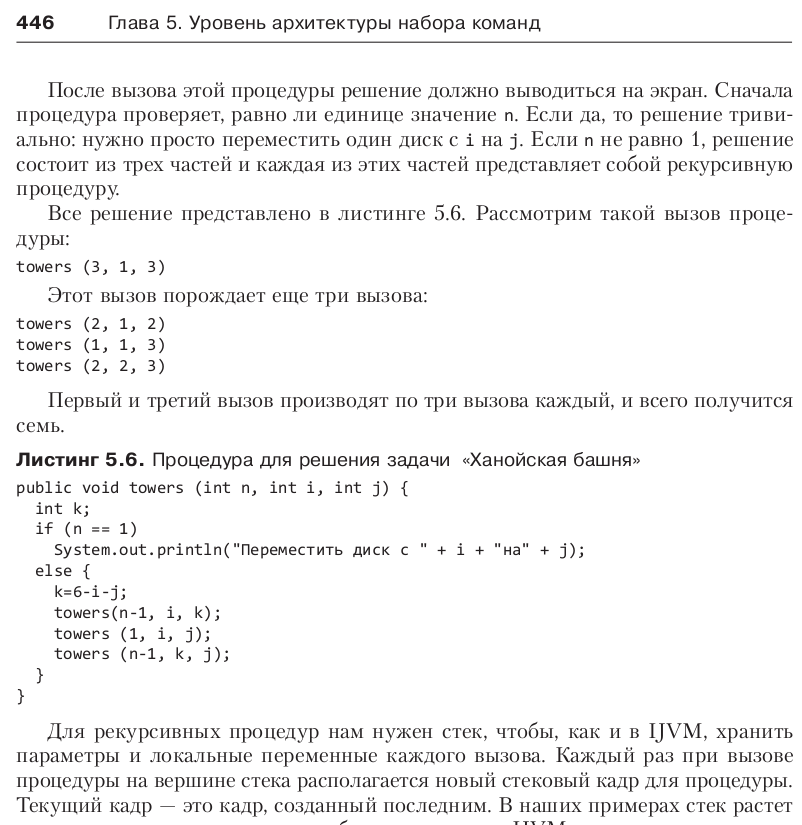
\includegraphics[width=\textwidth]{img/tan-aus.png}
\caption{\label{fig:tan-aus}Пример оформления листингов в~\autocite{TanAus2013}}
\end{figure}

Использовать внешние файлы (например, рисунки) можно и на \href{http://overleaf.com}{overleaf.com}: ищите кнопочку upload.

\subsection{Как оформить таблицу}

Для таблиц обычно используются окружения table и tabular --- см. таблицу~\ref{tab:widgets}. Внутри окружения tabular используются специальные команды пакета booktabs — они очень красивые; самое главное: использование вертикальных линеек считается моветоном.

\begin{table}
\centering
\caption{\label{tab:widgets}Подпись к таблице --- сверху}
\begin{tabular}{llr}
\toprule
\multicolumn{2}{c}{Item} \\
\cmidrule(r){1-2}
Животное  & Описание    & Цена (\$) \\
\midrule
Gnat      & per gram    & 13.65      \\
          & each        & 0.01       \\
Gnu       & stuffed     & 92.50      \\
Emu       & stuffed     & 33.33      \\
Armadillo & frozen      & 8.99       \\
\bottomrule
\end{tabular}
\end{table}

\subsection{Как набирать формулы}

\LaTeX{} is great at typesetting mathematics. Let $X_1, X_2, \ldots, X_n$ be a sequence of independent and identically distributed random variables with $\text{E}[X_i] = \mu$ and $\text{Var}[X_i] = \sigma^2 < \infty$, and let
$$S_n = \frac{X_1 + X_2 + \cdots + X_n}{n}
      = \frac{1}{n}\sum_{i}^{n} X_i$$
denote their mean. Then as $n$ approaches infinity, the random variables $\sqrt{n}(S_n - \mu)$ converge in distribution to a normal $\mathcal{N}(0, \sigma^2)$.

\subsection{Как оформлять списки}

Нумерованные списки (окружение enumerate, команды item)…

\begin{enumerate}
  \item Like this,
  \item and like this.
\end{enumerate}

\dots маркированные списки \dots

\begin{itemize}
  \item Like this,
  \item and like this.
\end{itemize}

\dots списки-описания \dots

\begin{description}
  \item[Word] Definition
  \item[Concept] Explanation
  \item[Idea] Text
\end{description}

\Conc

Помните, что на все пункты списка литературы должны быть ссылки. \LaTeX\ просто не добавит информацию об издании из bib"/файла, если на это издание нет ссылки в тексте. Часто студенты используют в работе  электронные ресурсы: в этом нет ничего зазорного при одном условии: при каждом заимствовании следует ставить соответствующую ссылку. В качестве примера приведём ссылку на сайт нашего института~\autocite{mmcs}.

Для дальнейшего изучения \LaTeX\ рекомендуем книгу Львовского~\autocite{Lvo2003}: она хорошо написана, хотя и несколько устарела.
Обычно стоит искать подсказки на
\href{http://tex.stackexchange.com/}{tex.stackexchange.com}, а также
читать документацию по установленным пакетам с помощью
команды
\begin{Verb}
texdoc имя_пакета
\end{Verb}
или на \href{http://ctan.org/}{ctan.org}.

% Печать списка литературы (библиографии)
\printbibliography[%{}
    heading=bibintoc%
    %,title=Библиография % если хочется это слово
]
% Файл со списком литературы: biblio.bib
% Подробно по оформлению библиографии:
% см. документацию к пакету biblatex-gost
% http://ctan.mirrorcatalogs.com/macros/latex/exptl/biblatex-contrib/biblatex-gost/doc/biblatex-gost.pdf
% и огромное количество примеров там же:
% http://mirror.macomnet.net/pub/CTAN/macros/latex/contrib/biblatex-contrib/biblatex-gost/doc/biblatex-gost-examples.pdf

\appendix
\ifthenelse{\value{worktype} > 1}{%
  \addtocontents{toc}{%
      \protect\renewcommand{\protect\cftchappresnum}{\appendixname\space}%
      \protect\addtolength{\protect\cftchapnumwidth}{\widthof{\appendixname\space{}} - \widthof{Глава }}%
  }%
}{
  \addtocontents{toc}{%
      \protect\renewcommand{\protect\cftsecpresnum}{\appendixname\space}%
      \protect\addtolength{\protect\cftsecnumwidth}{\widthof{\appendixname\space{}}}%
  }%
}

\section{Пример работы программы}

Здесь длинный листинг с примером работы.

\end{document}
